% ---------------------------------------------------------------------------
HTBAC serves as a software tool that enables the scalable and adaptive exploration 
of ensemble-based free energy studies. HTBAC is based on a 
co-design which integrates users i.e. domain experts and developers to elicit
requirements. 


% The co-design process is iterative. For example, certain features become available
% during the software lifetime which in turn can be used by domain experts to 
% build new algorithms that require such features. 


\subsection{Requirements}

HTBAC has three primary design requirements\@: (1) enable the scalable
execution of concurrent free energy protocols (2) abstract the complexity of 
building protocols, execution and resource management; and, (3) provide adaptive 
features (i.e., modifying the task-graph during runtime, based on previous tasks), 
to enable efficient protocols and effective resource sharing across protocols, 
without explicit resource management requirements.

Based on the requirements of the computational drug campaign which requires the 
ability to run multiple concurrent protocols in order to scale the number of 
drug candidates, this poses challenges in the 
workload management system and the runtime system (RTS) that support HTBAC. The 
RTS has to provide sustainable submission and tracking of heterogeneous protocols 
i.e. protocols that differ in computational requirements, as well as 
setup of execution environments and data management while preserving 
efficient resource utilization and minimal overhead. 

Usability plays an important role in the development of HTBAC, in order to provide
a flexible interface which enables users to easily scale the number of drug 
candidates and quickly prototype new algorithms and thereby new free energy 
protocols. 

Based on intermediate results during runtime, the control logic of the algorithm 
may decide to invest additional computational resources in more interesting  
candidates that can yield higher accuracy, while reducing resources for candidates
that have already met their accuracy threshold. HTBAC thereby requires an 
adaptive runtime systems that enables adaptive algorithms to maximize 
computational efficiency. 


\subsection{Design}

We model an application of HTBAC using the following user-facing constructs:

\begin{itemize}
  \item \textbf{Protocol:} A generic abstraction of a free energy protocol such
  as ESMACS or TIES. 
  \item \textbf{Simulation:} Simulation parameters that support and accompany 
  each protocol instance. 
  \item \textbf{Runner:} Cyber-infrastructure resource abstraction of the 
  application. 
\end{itemize}

The \textbf{Protocol} construct is the main abstraction of HTBAC. Each protocol
represents a physical system i.e. drug candidate. A protocol defines a
simulation pipeline composed of an ordered sequence of simulation steps. In
ensemble-based free energy protocol such as ESMACS or TIES, these simulation 
pipelines are replicated, where replicas differ by their parameter 
configurations. In ESMACS and TIES, replicas only differ by initial velocities, 
which are assigned randomly by the MD engine at the start of execution. By 
nature of ensemble applications, each replica within a protocol can execute its 
simulation pipeline independently. 

The \textbf{Protocol} class enables multiple instantiations of protocol types
such as ESMACS or TIES. Each protocol follows the same initial sequence of 
simulation steps i.e. minimization, equilibration and production simulation.  
Protocols differ only by their individual analysis step which typically follows 
production simulation and by the computational requirements,  
see figure X for a visual representation of the ESMACS and TIES workflows. 
In addition, the \textbf{Simulation} class specifies simulation parameters that
shape the protocol. The replica method defines the number of ensemble members 
for a given protocol instance, while the system method defines the input
configuration files necessary to execute the protocol instance. Moreover the 
\textbf{Simulation} class provides the granularity to specify individual 
parameters per replica, including the number of cores per replica, MD execution 
kernel and the length of each simulation step.

Some protocols require additional information. For 
example, the TIES protocol contains additional sampling parameters or   
$\lambda$ windows. Moreover, the \textbf{Simulation} class exposes a 
workflow method which enables the user to codify new algorithms, or modify
an existing protocol such as specifying additional equilibration or analysis 
steps. 

Once the protocols and simulation parameters 
are defined, they are passed to the \textbf{Runner} class where the user defines 
the resource requirements including cyber-infrastructure and duration of the 
application as well as additional flags for adaptive execution which are passed 
down by the \textbf{Runner} to the workload management and runtime systems. 
Figure X shows the control flow representation of HTBAC. 


% For TIES, where each protocol  corresponds to a single 
% physical system. The TIES protocol 
% object enables the user to select a physical system, number of replicas, 
% core allocation per replica, and $\lambda$ windows to sample. 
% Figure~\ref{fig:pst} provides the visual implementation of the TIES protocols 
% into the PST model.

\subsection{Implementation}

HTBAC is implemented in Python, and uses RADICAL-Cybertools (RCT) to provide 
ensemble-execution capabilities and a runtime system to execute protocols. 
The RCT are middleware building blocks~\cite{review_bb_2016} engineered to 
support extensible and scalable workflows across diverse computing
platforms~\cite{turilli2017comprehensive}. HTBAC rests on two primary RCT 
components, Ensemble Toolkit (EnTK) and RADICAL-Pilot (RP). 

\begin{figure}
  \centering
   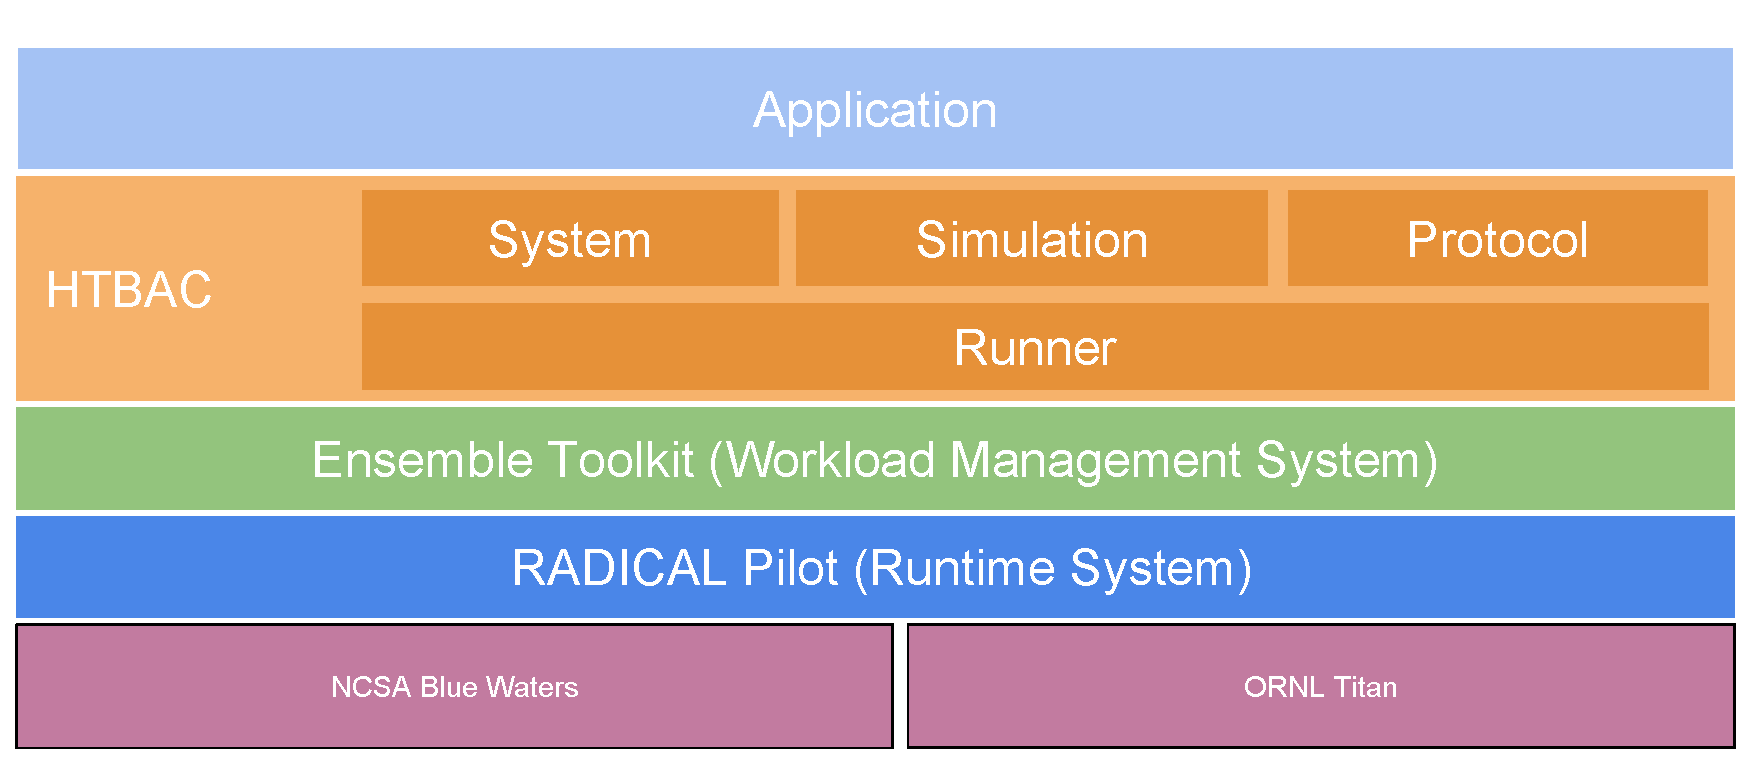
\includegraphics[width=\columnwidth]{figures/building_blocks.pdf}
  \caption{Layered architecture of HTBAC, EnTK, and RP. The HTBAC API exposes 
  the Protocol component. Current protocols supporting the use cases include 
  ESMACS and TIES. EnTK serves as the workload execution system. RADICAL-Pilot 
  serves as the runtime system.}
\label{fig:blockdiagram}
\end{figure}

Figure~\ref{fig:blockdiagram} shows a visual block diagram representation of 
HTBAC and the underlying building blocks. 

\subsection{Workload Management and Runtime System}

EnTK simplifies the process of creating ensemble-based applications with
complex coordination and communication requirements. The EnTK API exposes the
PST model which consists of three components: \textbf{Pipeline},
\textbf{Stage}, and \textbf{Task}. HTBAC promotes binding affinity {\bf
Protocols} as the user-facing construct, and uses the programming model
defined by the Pipeline, Stage and Tasks model to express a specific
protocol. 

% Each HTBAC application aggregates one or more protocols. A workflow is comprised 
% of $N_P$ instances of the P$^{th}$ protocol. 

% each stage is a computational \textbf{task}, and the
% ordered aggregation of these stages alongside their dependencies as a
% \textbf{pipeline}~\cite{power-of-many17}. 

% Sets of tasks with dependencies that determine the order of their execution are usually referred to as “workflows”. 

% In section \ref{sec:science-drivers}, we 
% described two examples of ensemble-based protocols for computing binding 
% affinities.

Once the workflow is described, protocols are translated into EnTK pipelines, and 
are submitted to EnTK's \textbf{Application Manager} which sets up multiple 
processes, threads and a RabbitMQ message queue for communication.
EnTK identifies tasks which have satisfied dependencies and can be executed
concurrently. EnTK's \textbf{Execution Manager} uses the underlying runtime
system, RADICAL-Pilot to execute the tasks on specific target resources.

EnTK converts the set of pipelines into a set of tasks called compute unit 
descriptions and submits them to RP. In addition, HTBAC passes the computational
requirements to EnTK which creates a resource request including walltime, cores, 
queue, and user credentials. EnTK converts this resource request into a pilot 
that RP submits to a HPC machine. Once the pilot becomes active, it pulls 
compute unit descriptions in bulk from a database, executing them on the pilot 
resources. 

\begin{figure}
  \centering
   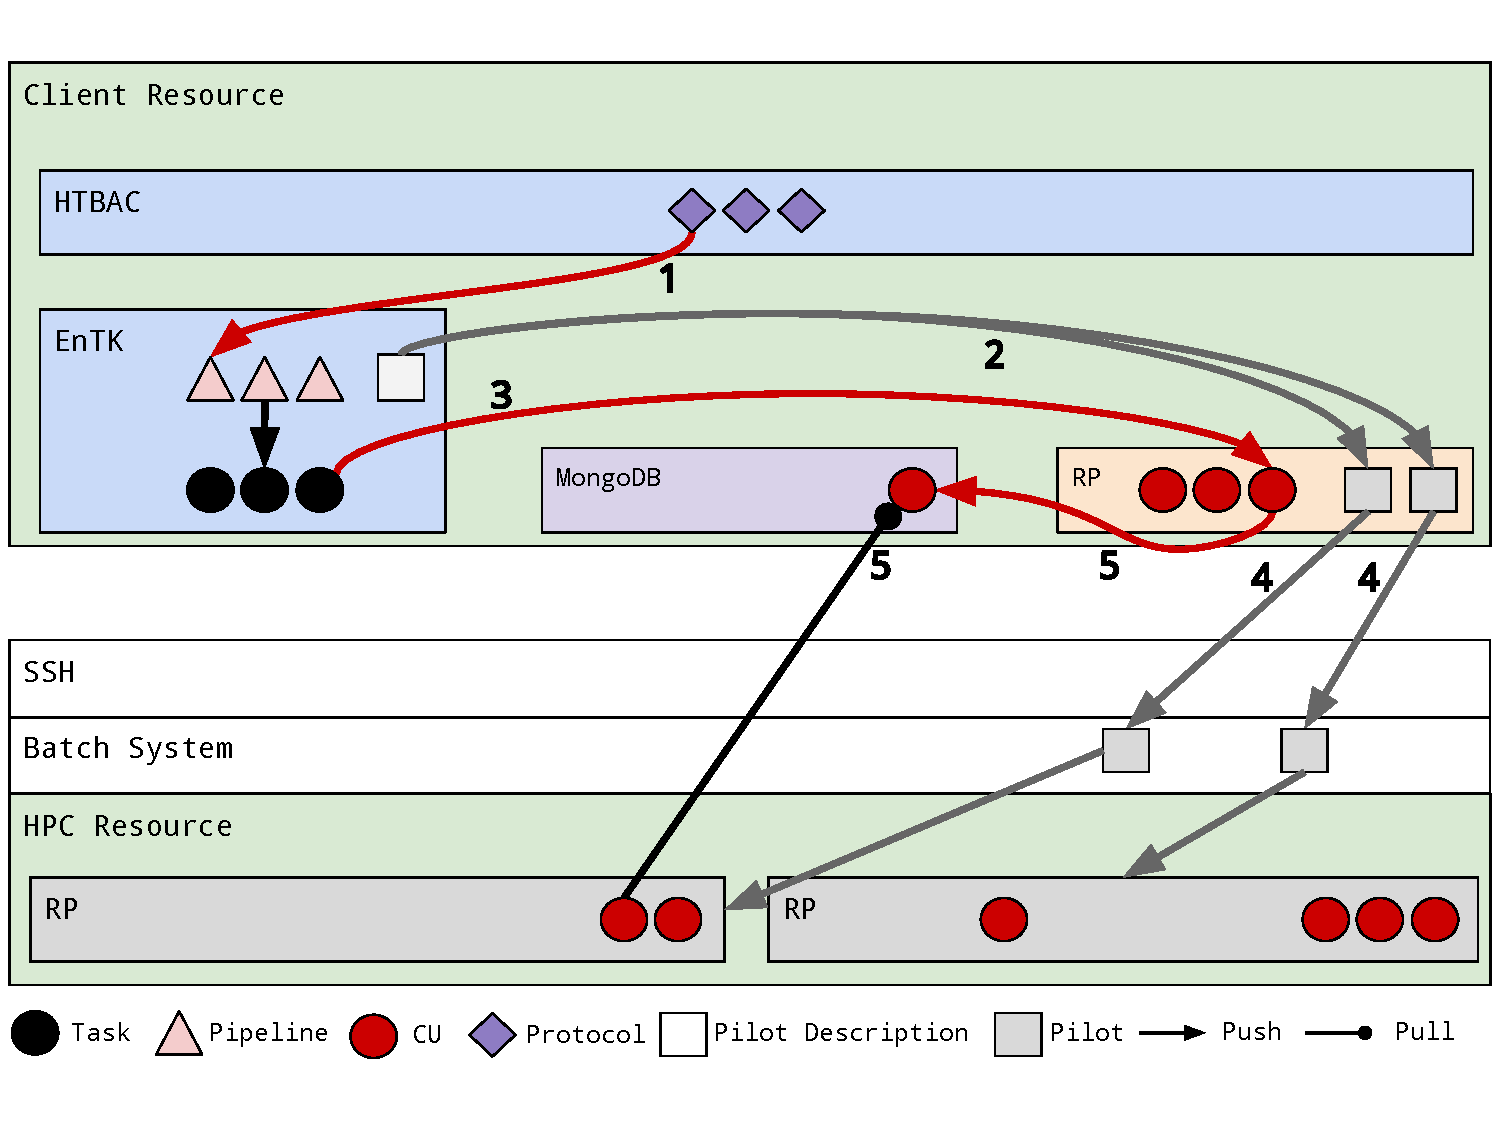
\includegraphics[width=\columnwidth]{figures/ht-bac-rp_integration.pdf}
  \caption{Ensemble Toolkit (EnTK) and RADICAL-Pilot (RP) architecture and 
  execution model.}
\label{fig:integration}
\end{figure}

% Consistent with EnTK's programming model, HTBAC also uses the PST model to
% express {\bf Protocols}.

% Each protocol contains multiple stages with simulations and analysis tasks
% interspersed, in the most general case. 


% programming model (that are consistent with the EnTK) to enable the user 





% HTBAC rests upon established middleware solutions~\cite{review_bb_2016},
% validated runtime abstractions~\cite{turilli2017comprehensive} for scalable
% execution, and customizes them for the computation of binding free energies. 


% HTBAC derives many of the advantages of
% a lightweight, flexible domain specific workflow layer from its use of
% RADICAL-Cybertools (RCT) which are functionally well-defined and delineated
% middleware building blocks. RCT~\cite{review_bb_2016} are engineered to
% support extensible and scalable workflows across diverse computing platforms.
% The two primary RCT components that HTBAC depends upon are the Ensemble
% Toolkit (EnTK) and RADICAL-Pilot (RP). 


% (so far, a
% workflow entails a maximum value of $P = 2$ and $N_P$=16, but in future work P
% will be greater $>$ 2).


% protocol, a user can scale protocol instances to study as many physical systems as
% desired.

% The specification of protocols and their parameters are passed by the user to
% the \textbf{Runner Handle} which translates the request to EnTK.

% In Section \ref{sec:related-work} we highlighted how an ensemble
% simulation approach can both aid sampling and improve uncertainty
% quantification for free energy calculations. Despite these crucial advantages,
% it remains non-trivial for field researchers to write biosimulation
% applications that involve individual protocols supporting multiple replicas,
% and by extension multiple protocols. With HTBAC, this burden is minimized by
% specifying the number of concurrent instances of the \textbf{Protocol} object.
% Moreover, the ability to generate multiple protocol instances enables the user
% to investigate a range of physical systems (i.e., drug candidates)
% concurrently.

% HTBAC allows the simple expression and concurrent execution of multiple
% distinct protocols, thereby enabling concurrent screening of drug candidates.
% HTBAC not only simplifies the expression of complex binding affinity
% protocols, but also provides hitherto unavailable capabilities, viz., the
% adaptive execution of these protocols, without any additional programming
% burden. 

Explain adaptive API and how it is passed to EnTK


% In turn, our adaptive execution implementation at the WMS focuses on
% supporting generality of adaptive workflows at the inter and intra-protocol
% level.

\begin{figure}
  \centering
   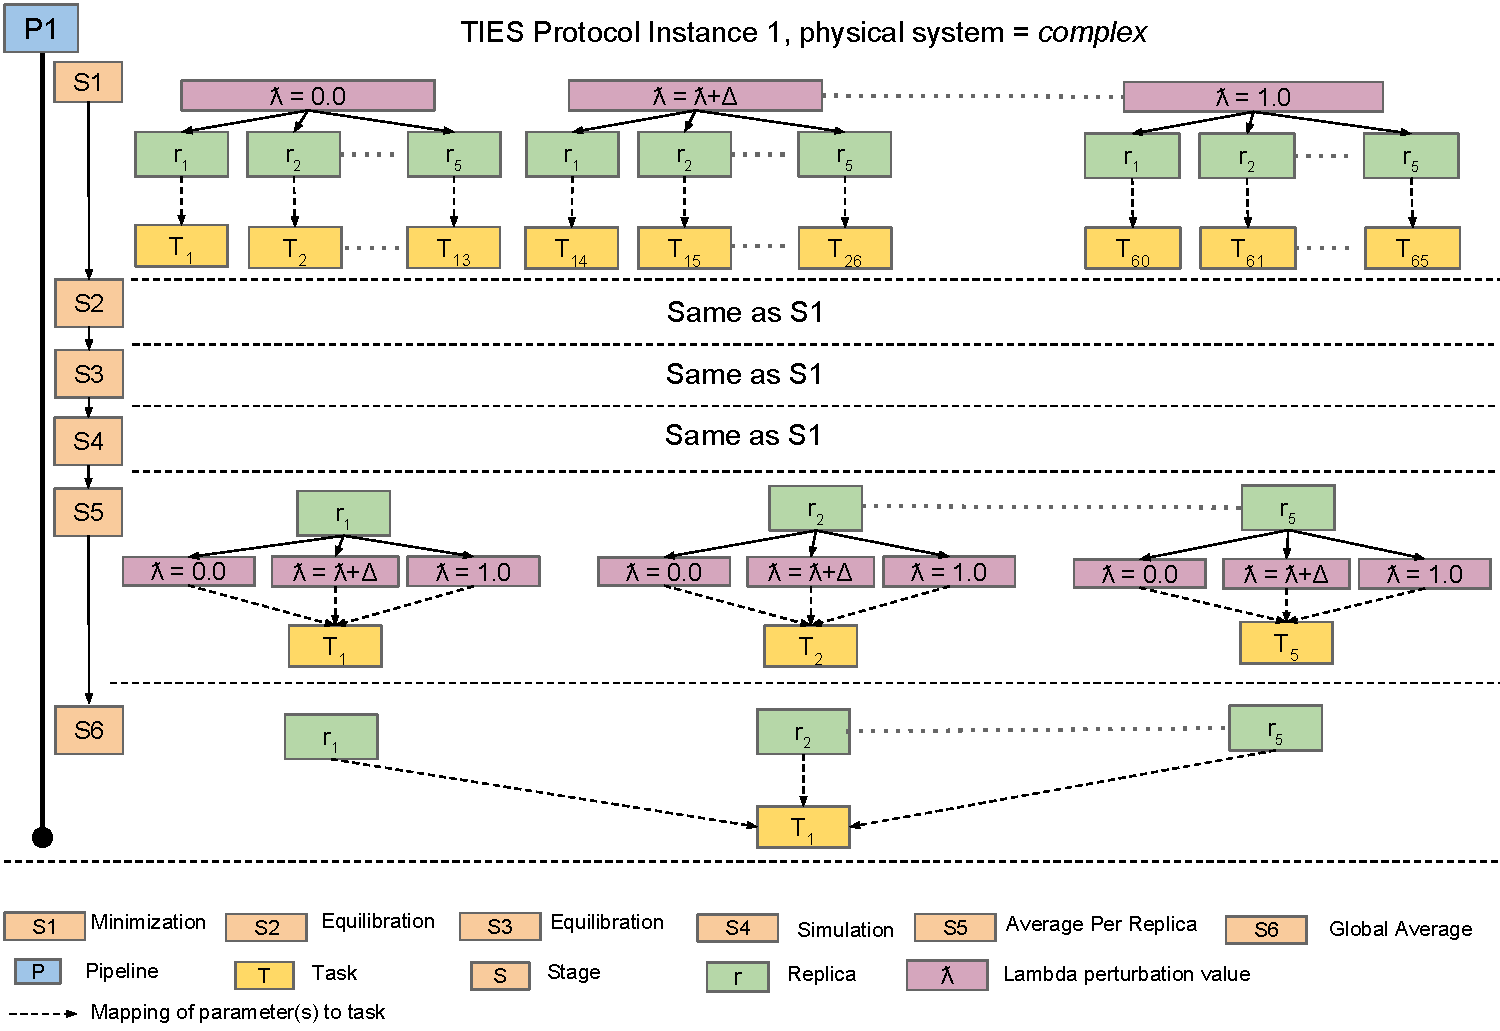
\includegraphics[width=\columnwidth]{figures/_TIES_EnTK_implementation.pdf}
  \caption{TIES protocol expressed using the EnTK PST model. Each protocol 
  instance maps to a single Pipeline, comprised of Stage(s) which maintain 
  temporal order. Each Stage executes $n$ tasks, where $n$ represents the 
  number of unique lambda-replica combinations.}
\label{fig:pst}
\end{figure}


% \subsection{Scalability}

% Each protocol instance studies a single physical system 
% i.e. drug candidate. By extension, the user is able to scale the number of 
% concurrent protocol instances and therefore explore multiple concurrent drug 
% candidates. 

\subsection{Adaptivity}

In section \ref{sec:science-drivers}, we described a particular type of
adaptivity within TIES that would enable the simulation to reach
convergence earlier. Adaptive execution requires changes to the task graph 
during runtime, capabilities that are supported by the RCT runtime 
layers~\cite{power-of-many17}.

The TIES adaptive workflow decides, post-mortem, about the placement
of new lambda windows for the next set of simulations. In turn, the workflow
makes runtime decisions to the number of tasks in the task graph. This type of 
adaptivity in the workflow requires as task-count and task-attribute 
adaptivity~\cite{adaptivebiomolecular}. 

HTBAC monitors the output results from the completed tasks
during runtime, and redefines the existing workflow by adding more $\lambda$
windows. A boolean results generated at the end of a pipeline defines a criteria
of whether or not to spawn additional tasks. 
% Spawning of new task contribute
% to task count adaptivity and task attribute adaptivity. 
% Using EnTK, HTBAC creates the necessary set of new tasks. 

The \textbf{Application
Manager} in EnTK signals RP to bypass termination of the pilot and instead
keep the session alive, as long as additional tasks are submitted. As the
number of tasks grow during runtime, the ratio of core-to-task will fluctuate.
HTBAC exposes the core allocation per task, and allows the user control to
pre-specify resource requirements of additional tasks.

% ---------------------------------------------------------------------------


%\jhanote{Is this specific to the TIES protocol or to the protocol class. Needs
%clarification.}
%The same approach has been expanded to facilitate the creation of
%sub-ensembles where the simulation configuration is altered programatically.
%An example of this is the implementation ofthe TIES protocol,
%where the user controls the $\lambda$ parameter values used in simulatios to
%control which hybrid system states are sampled.

%A parameter, $\lambda \in [0, 1]$ is set for values between extremes and a
%simulation has to be run for every $\lambda$ value. The values form a function
%of energy and are integrated to obtain the desired results, the
%\emph{relative} binding free energy.

%\subsubsection{System}

%Systems This allows for multiple systems to be tested in the same
%\emph{single} run. A common scenario is the calculations of the binding
%affinity of a set of ligands with the same protein. System itself is just a
%collection of file paths pointing to descriptions of the system, like the
%system structure, topology etc. This class also provides the core/node
%requirments per single run, and reads some of the system descriptions from
%files to fill in the configuration settings.

%The Pipeline-Stage-Task (PST) framework developed by the Radical team
%(cite), and the Ensemble Toolkit (EnTK) built on top of it, offers a
%flexible way to express the molecular dynamics simulation workflows present
%in academia (cite) in terms of the radical pilot execution environment. Here
%we present a proposed mapping between the two (the PST and the MD layers)
%that is both simulation engine and protocol agnostic and allows for the
%compact expression of ensembles frequently used in binding affinity
%calculations.

%\subsection{Overview}

%The framework, called High Throughput Binding Affinity Calculator (HT-BAC),
%a python library, is made up of the following components: Workflow, Step,
%Ensembles and Simulation. These four object are all that is neccessary to
%describe the complex binding affinity caluculations in a generic way.

%\subsection{Workflow}

%The highest level abstraction is the Workflow. It is a container for the
%sequential units that are the simulation steps themselfs, and also contains
%meta-information about the job, like the resource description that the job
%will be running on, the total number of cores (nodes) required to fullfil
%the needs of the simulations and profiling mechanims to measure execution
%time.

% ---------------------------------------------------------------------------
%\jhanote{I don't these "description" should be subsections. Consider
%"\paragraph{}"}

%\subsection{Step}

%\jhanote{what is a step? It is unclear to the reader. Is "step"  construct
%within HTBAC or is this just a description of the pipeline?}

%The workflow containts an ordered list of \emph{steps}. Steps give
%\jhanote{order?} orderd to the basic building blocks of binding affinity
%calculations. Usually they are (i) minimization (some form of local
%optimization of atom coordinates), (ii) heating, (iii) equilibration and (iv)
%production run.

%Additionally there is one or more steps of analysis at the end. The key
%point, is that these steps \emph{have} to be run consecutively, as they are
%dependent on the previous one. This is ensured by the \texttt{Stage} objects
%of EnTK\@. Each step has list of \texttt{Ensemble}s and a \texttt{Simulation}
%object.

% ---------------------------------------------------------------------------

%$\subsection{Adaptability}

%Once we tackle the barrier between the local workflow creation and the remote
%execution, new features become availble, and readily usable by scientists.
%Intraprotocol adaptability is one such new feature.

% ---------------------------------------------------------------------------

% \subsubsection{Intraprotocol adaptability}

%while conceptually simple, tradiational execution patters used in academia
%makes this very hard. In HTBAC variables like replica size, specific lambda
%windows or simulatable system are settable on demand, the execution of which
%is automatically handeled by the library. To illustrate: a common scenario is
%the non adequate convergence of the statistical results after running a given
%number of replicas. In HTBAC the replica number can be changed, rerun and the
%results reevaluated. Additionally, logic can be written, to dynamically add
%more replicas until a given convergence tolerance has been reached.
